\chapter{Setup} % <<< -------------------------------------------------------- %
\label{ch:userguide:setup}
% ---------------------------------------------------------------------------- %

Assuming the STEMlab board at hand was delivered with an SD card containing the correct Linux image, the setup only requires the following steps:

\begin{enumerate}
    \item Insert the SD card coming with the board (NOTE: Check that the SD card has the right side up to make pin contact).
    \item Connect the board physically to the network.
    \item Connect the board to the power supply.
    \item Call the boards IP and the right port (eg. https://10.84.130.54:50090) in a browser of preference (for best results use Chrome 61.0 and above). Figure~\ref{fig:userguide:popup:warn} shows an example how to do this.
    \item A notice that a popup has been blocked should appear. Select "Always allow popups from this application." or similar and reload the previously called page. Figure~\ref{fig:userguide:popup:yes} illustrate the necessary setting.
    \item A popup tab should now contain the scope and automatically connect to the STEMlab's webserver. Figure~\ref{fig:userguide:running} shows a running scope.
\end{enumerate}

If it is unknown wether the SD card was delivered with a prebuilt image, it can be assumed that it was so and the board can be powered. If the LED farthest away from the ports flashes orange with \SI{2}{\Hz}, the SD card is fine.

If the SD card does not contain a prebuilt image, the Devguide should be consulted in Section~\ref{TODO:} on how to acquire or build an image.

\begin{figure}
    \centering
    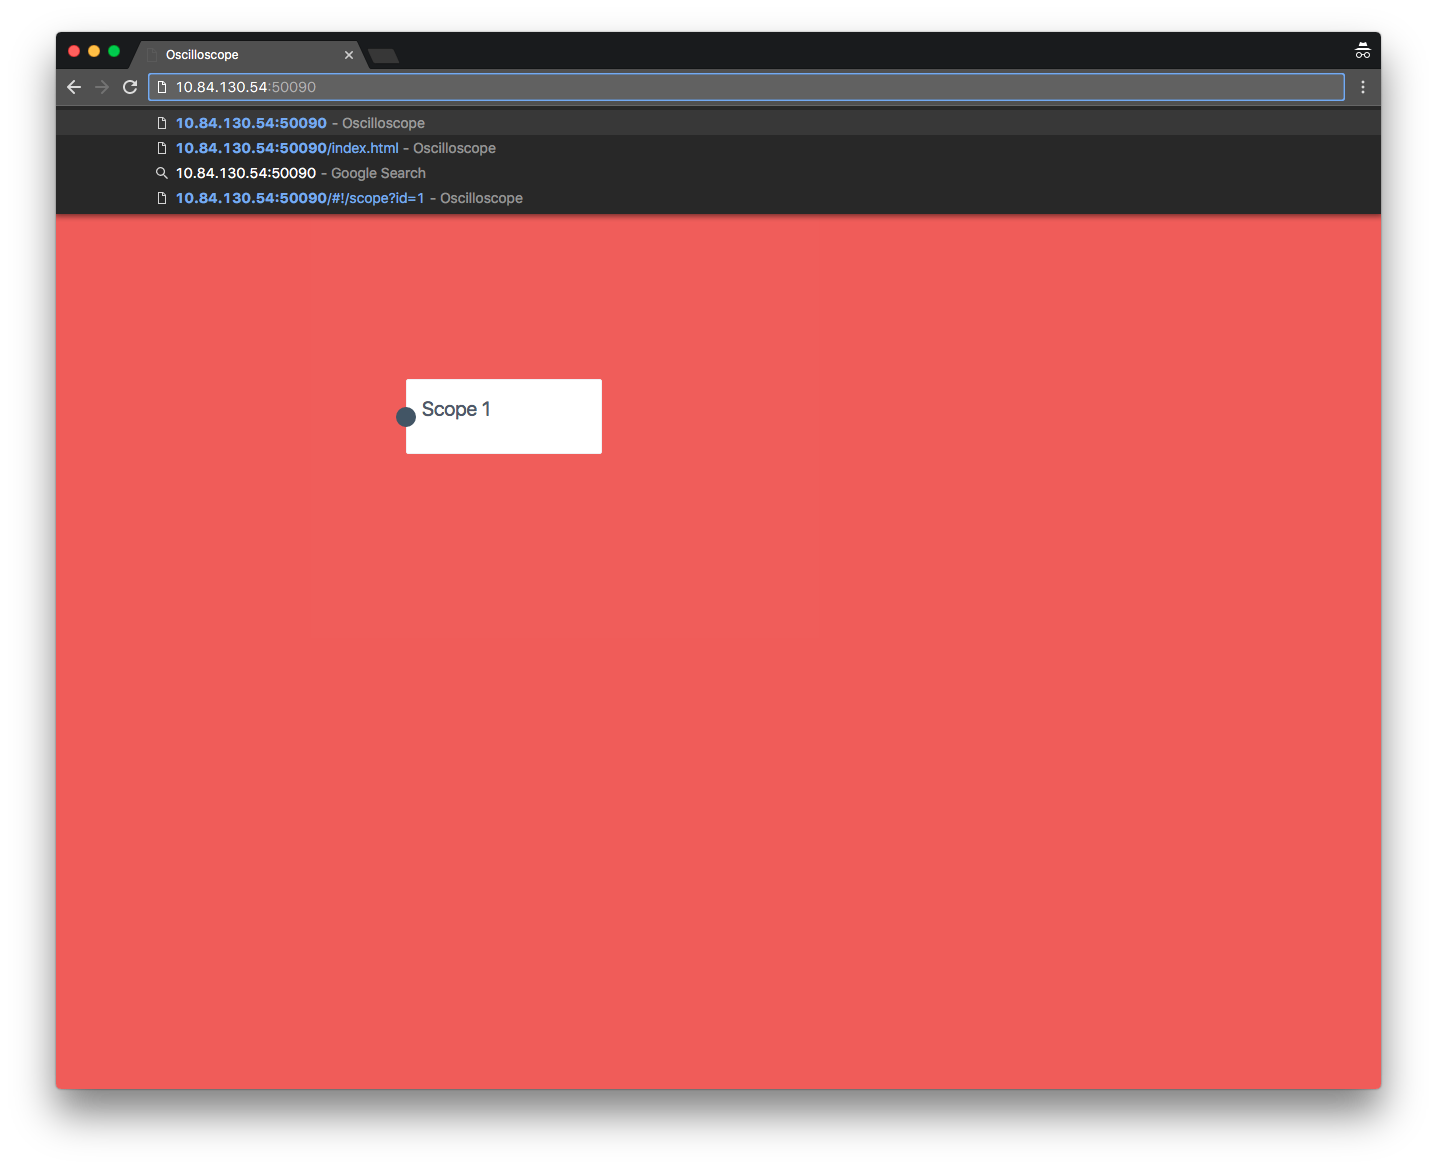
\includegraphics[width=1\textwidth]{images/userguide/url}
    \caption[Entering the URL]{%
        Using a browser and the correct URL to run the scope application on the STEMlab.
    }
    \label{fig:userguide:url}
\end{figure}

\begin{figure}
    \centering
    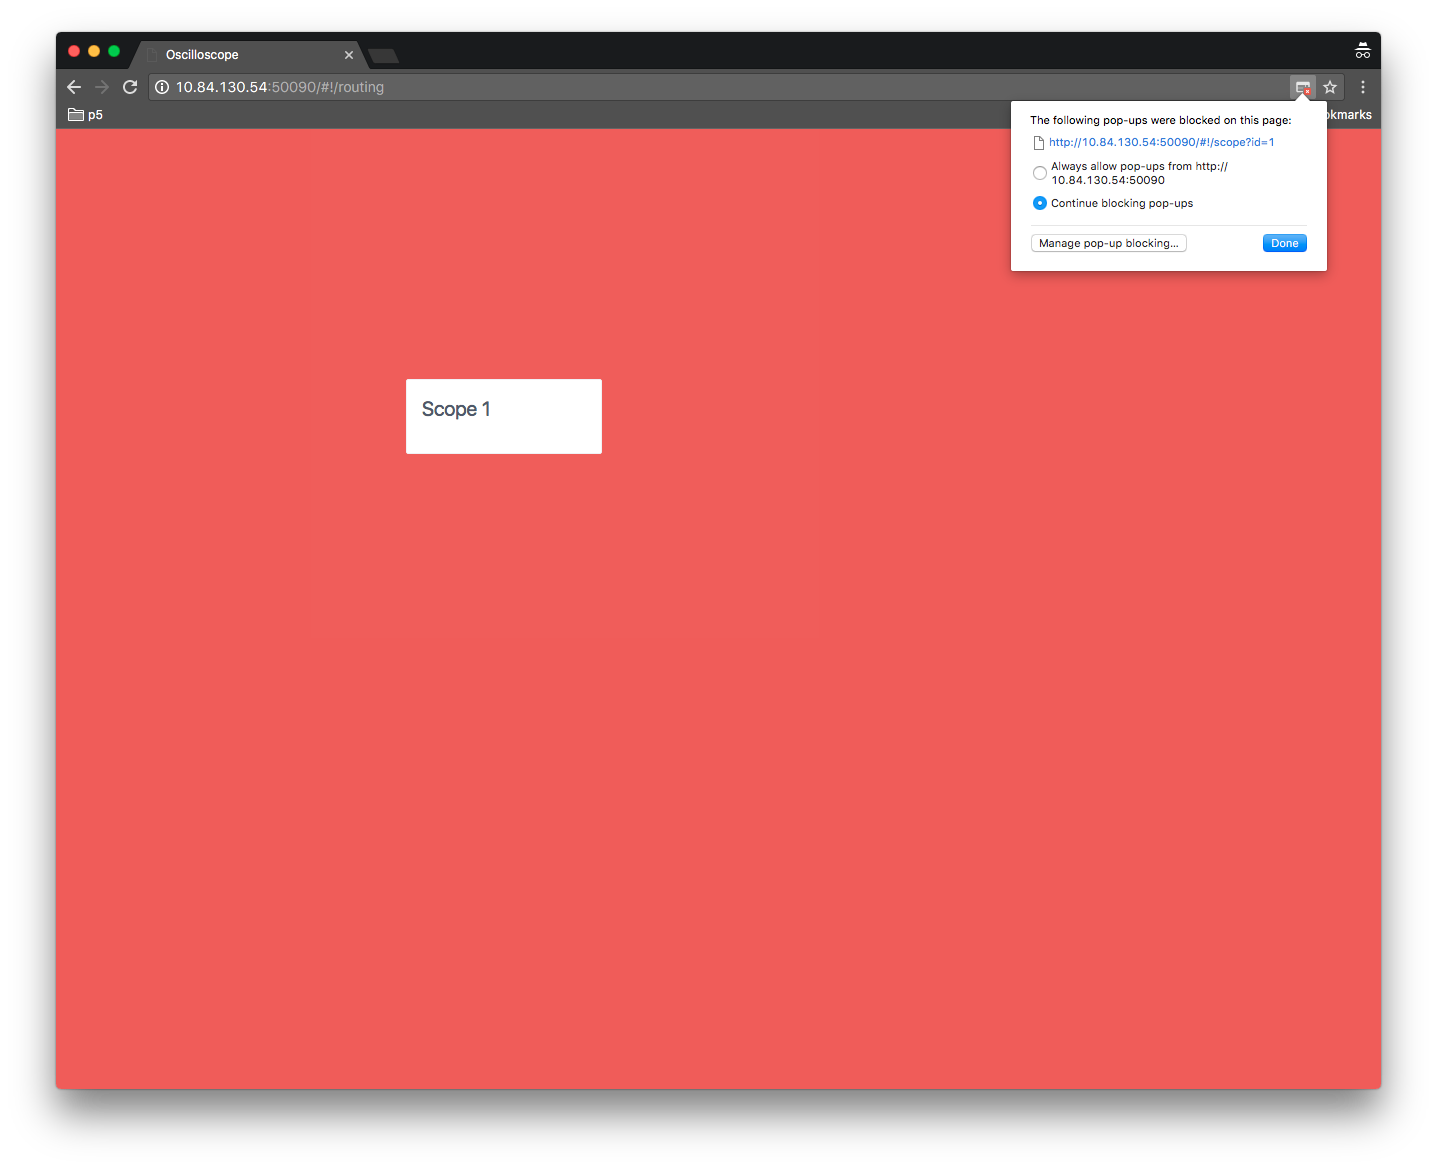
\includegraphics[width=1\textwidth]{images/userguide/popup_warn}
    \caption[The popup warn popup]{%
        The browser warns about a popup the site has tried to open.
    }
    \label{fig:userguide:popup:warn}
\end{figure}

\begin{figure}
    \centering
    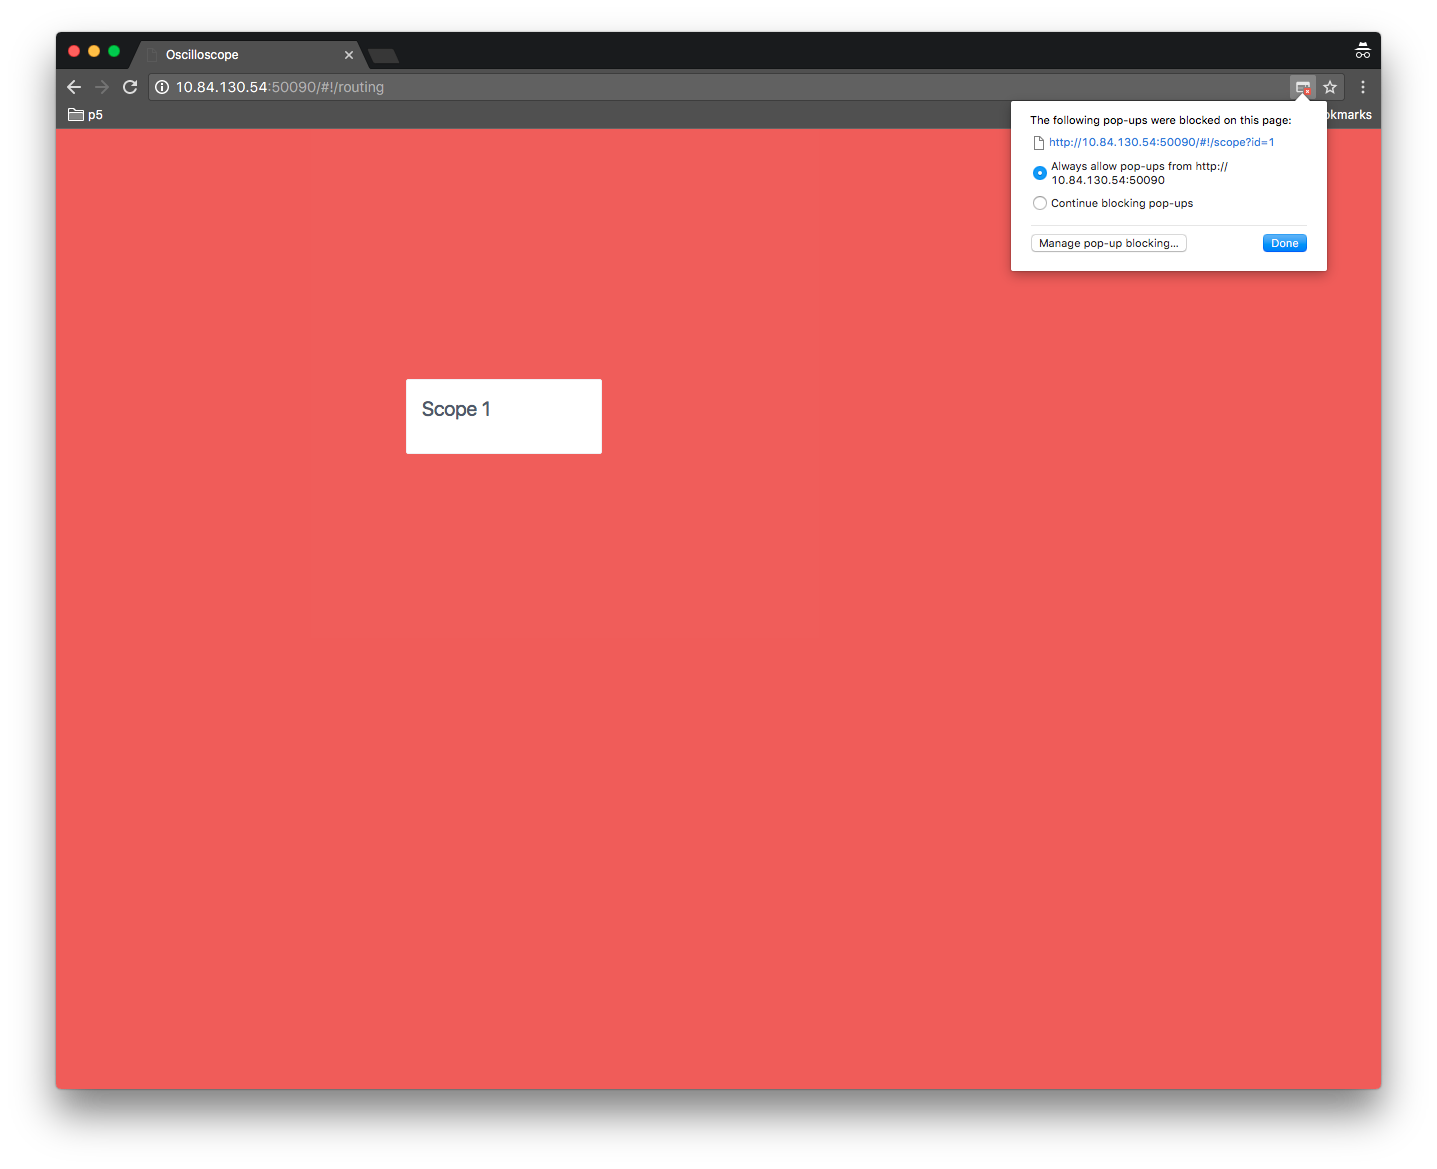
\includegraphics[width=1\textwidth]{images/userguide/popup_yes}
    \caption[Accept popups in the future]{%
        Let the browser accept popups in the future.
    }
    \label{fig:userguide:popup:yes}
\end{figure}

\begin{figure}
    \centering
    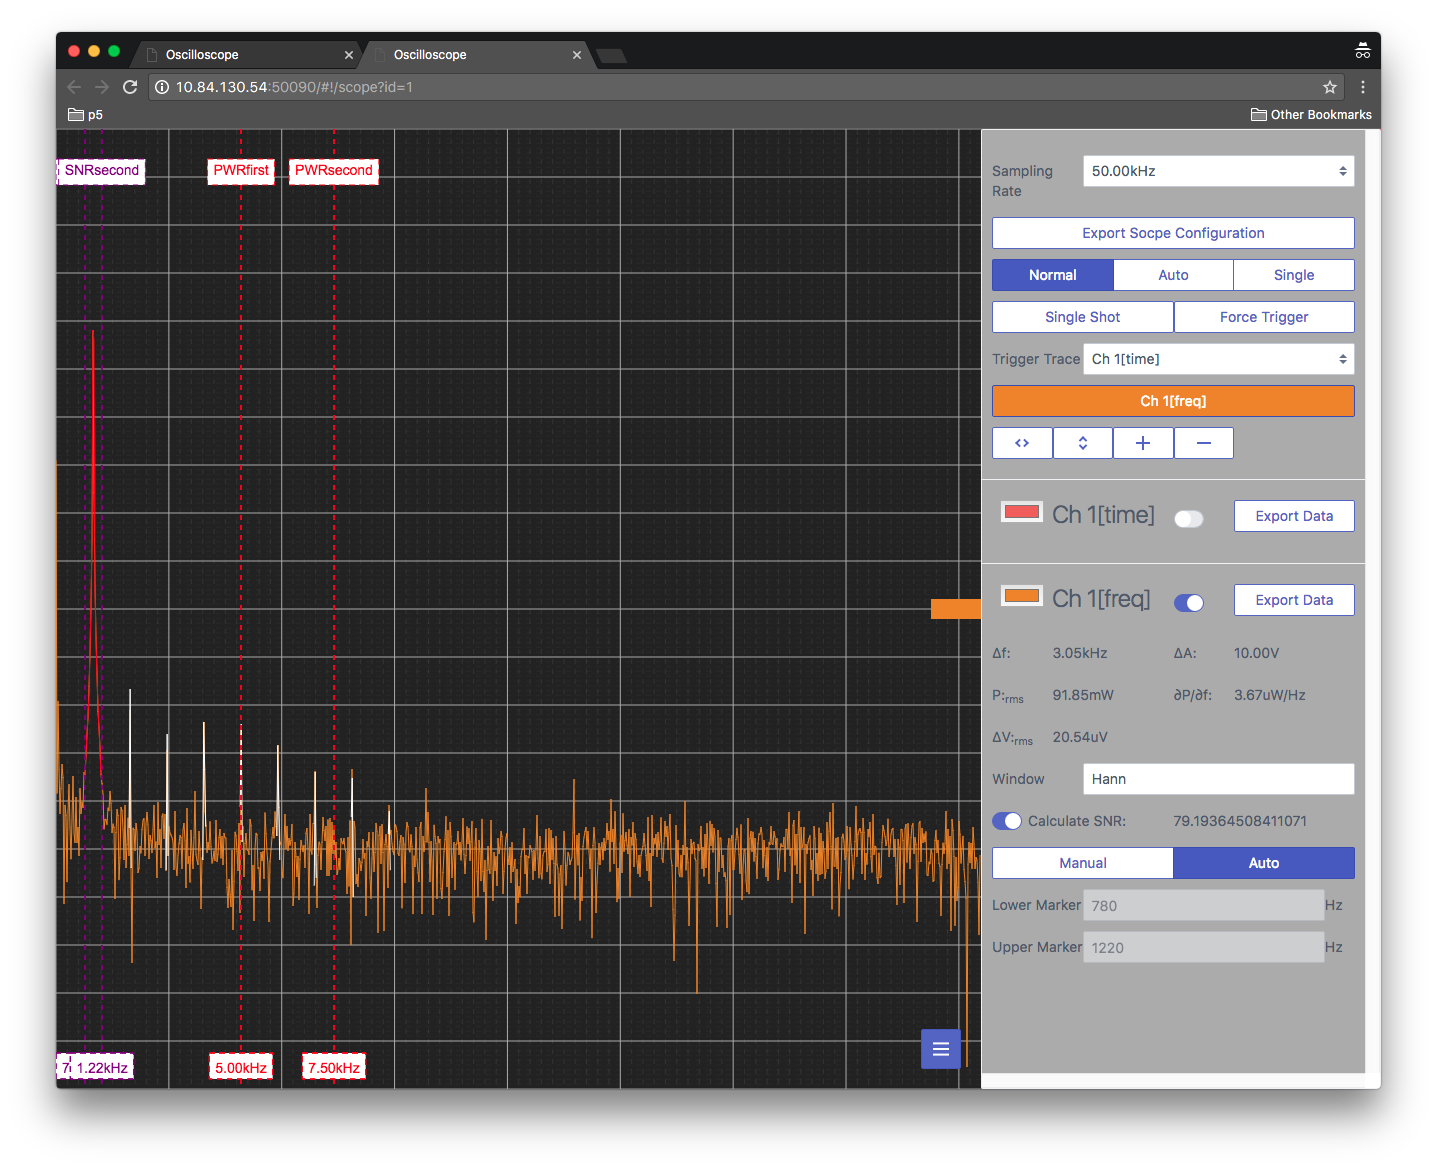
\includegraphics[width=1\textwidth]{images/userguide/running}
    \caption[Running the scope]{%
        The running scope after everything was set up properly.
    }
    \label{fig:userguide:running}
\end{figure}

%>>>
\chapter{Operation} % <<< ---------------------------------------------------- %
\label{ch:userguide:operation}
% ---------------------------------------------------------------------------- %

%>>>

%^^A vim: foldenable foldcolumn=4 foldmethod=marker foldmarker=<<<,>>>
